\documentclass[border=10pt]{standalone}
\usepackage[svgnames]{xcolor}
\usepackage{amsmath}
\usepackage{pgfplots}
\pgfplotsset{compat=newest}
\usepackage[sfdefault]{FiraSans}
\usepackage{FiraMono}
\renewcommand*\familydefault{\sfdefault}
\begin{document}
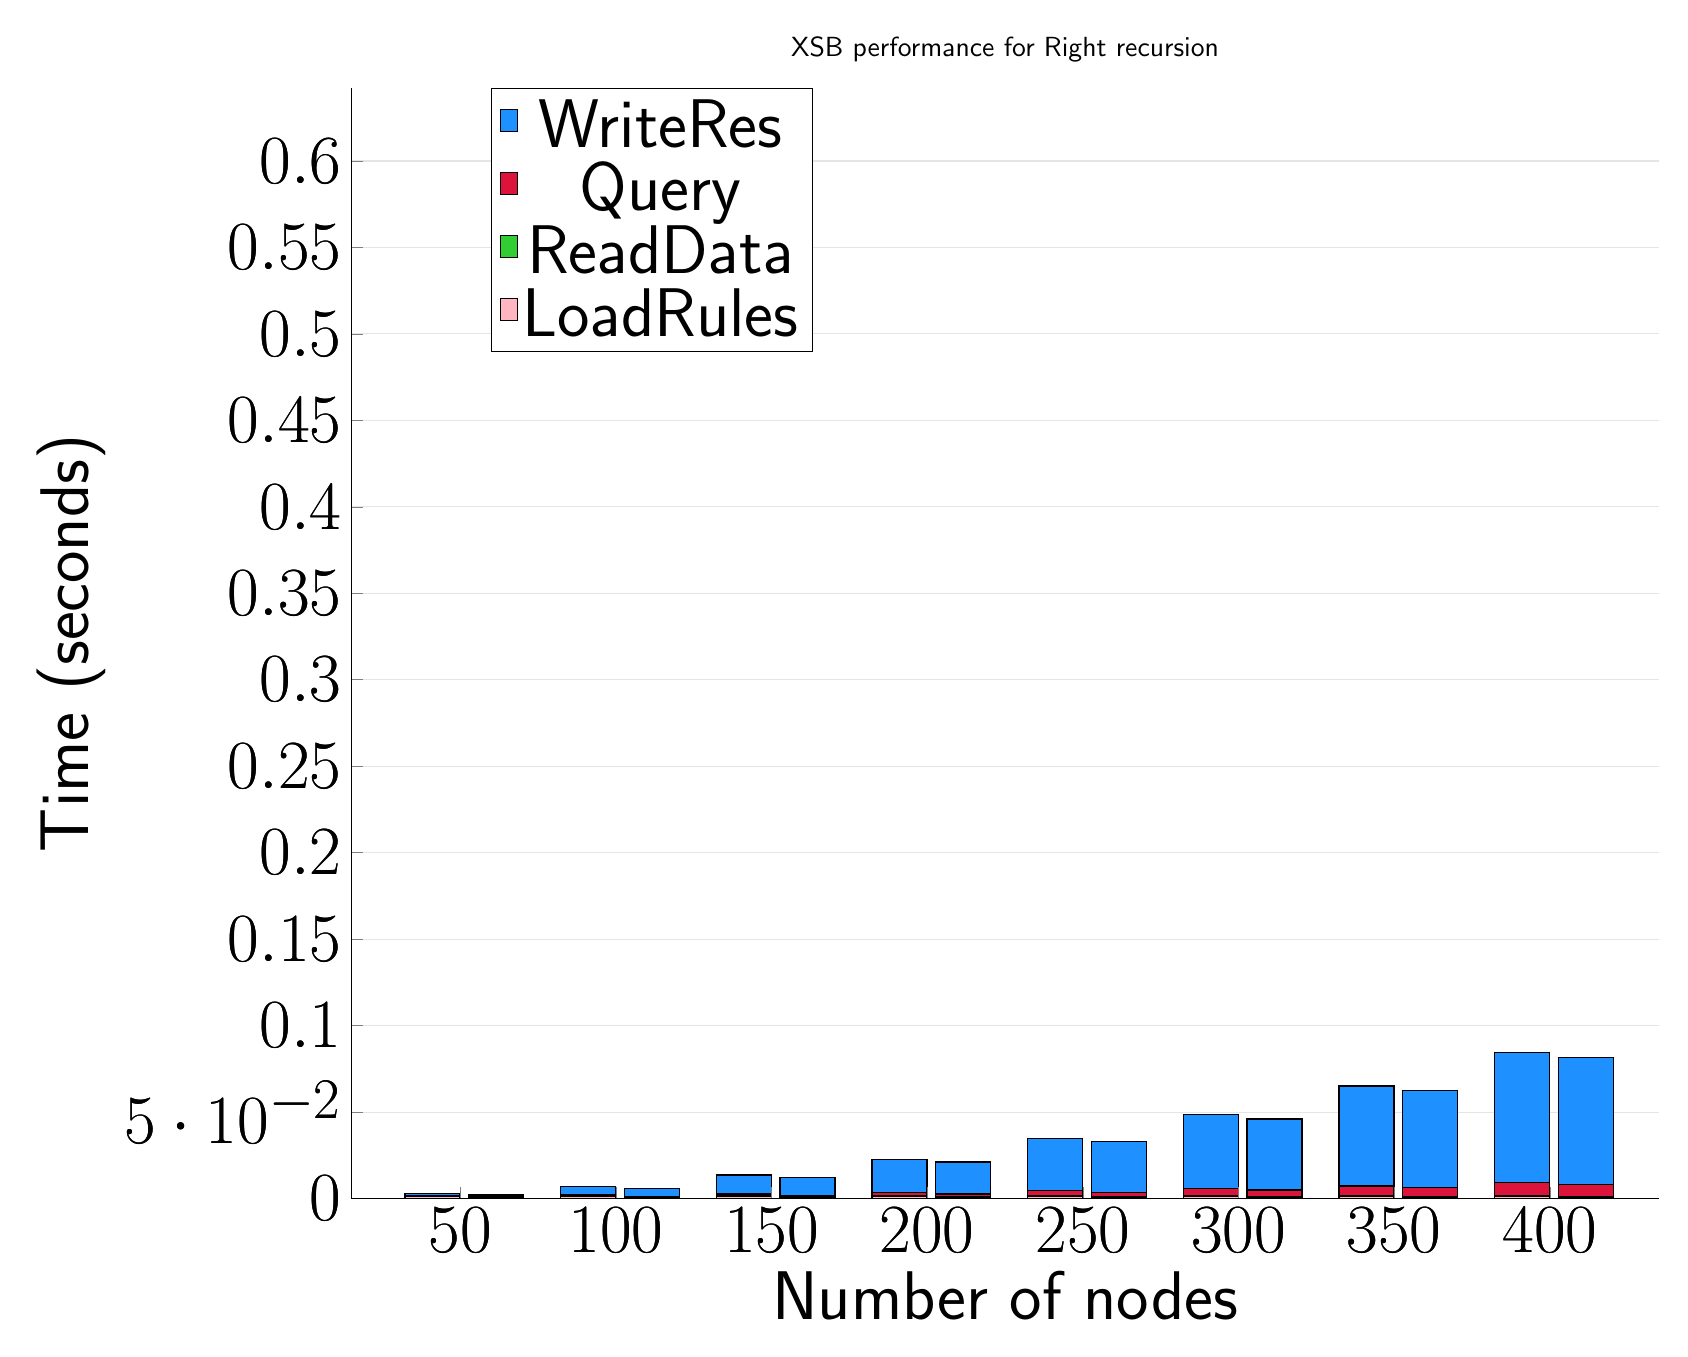
\begin{tikzpicture}
	\begin{axis}[
			ybar stacked,
			title={XSB performance for Right recursion},
			bar shift=-10pt,
			width=1.5\textwidth,
			bar width=0.7cm,
			ymajorgrids, tick align=inside,
			major grid style={draw=gray!20},
			xtick=data,
			ymin=0, ymax=0.6422704648971556,
			axis x line*=bottom,
			axis y line*=left,
			enlarge x limits=0.1,
			legend style={
					at={(0.23, 1)},
					anchor=north,
					legend columns=1,
					font=\Huge,
				},
			ylabel={Time (seconds)},
			xlabel={Number of nodes},
			label style={font=\Huge},
			tick label style={font=\Huge},
		]
		\addlegendimage{fill=DodgerBlue, draw=black, line width=0.2pt}
		\addlegendentry{WriteRes}
		\addlegendimage{fill=Crimson, draw=black, line width=0.2pt}
		\addlegendentry{Query}
		\addlegendimage{fill=LimeGreen, draw=black, line width=0.2pt}
		\addlegendentry{ReadData}
		\addlegendimage{fill=LightPink, draw=black, line width=0.2pt}
		\addlegendentry{LoadRules}
		\addplot +[fill=LightPink, draw=black, line width=0.5pt] coordinates {
				(50, 0.0010922431945800779)
				(100, 0.001082730293273926)
				(150, 0.001059103012084963)
				(200, 0.001044893264770508)
				(250, 0.001038193702697753)
				(300, 0.001049661636352539)
				(350, 0.001034712791442871)
				(400, 0.0010788679122924812)
			};
		\addplot +[fill=LimeGreen, draw=black, line width=0.5pt] coordinates {
				(50, 0.00041475296020507794)
				(100, 0.0004257917404174803)
				(150, 0.00047218799591064464)
				(200, 0.0005388736724853516)
				(250, 0.000576424598693848)
				(300, 0.0006610393524169922)
				(350, 0.00070652961730957)
				(400, 0.0007525205612182619)
			};
		\addplot +[fill=Crimson, draw=black, line width=0.5pt] coordinates {
				(50, 0.0001422882080078127)
				(100, 0.0004879951477050783)
				(150, 0.001070404052734375)
				(200, 0.0019100427627563484)
				(250, 0.0029209613800048827)
				(300, 0.004212117195129394)
				(350, 0.005639338493347168)
				(400, 0.007395529747009276)
			};
		\addplot +[fill=DodgerBlue, draw=black, line width=0.5pt] coordinates {
				(50, 0.0013857364654541013)
				(100, 0.004858899116516114)
				(150, 0.010937952995300296)
				(200, 0.01912033557891847)
				(250, 0.030271863937377918)
				(300, 0.042554259300231934)
				(350, 0.05776228904724123)
				(400, 0.07530307769775392)
			};
	\end{axis}
	\begin{axis}[
			ybar stacked,
			bar shift=13pt,
			width=1.5\textwidth,
			bar width=0.7cm,
			ymajorgrids, tick align=inside,
			major grid style={draw=none},
			xtick=data,
			ymin=0, ymax=0.6422704648971556,
			axis x line*=none,
			axis y line*=none,
			enlarge x limits=0.1,
			label style={font=\Huge},
			tick label style={font=\Huge},
		]
		\addplot +[fill=LightPink, draw=black, line width=0.5pt] coordinates {
				(50, 0.0006195000000000006)
				(100, 0.0006214000000000003)
				(150, 0.0006144)
				(200, 0.0006048999999999999)
				(250, 0.0006013999999999999)
				(300, 0.0006062999999999999)
				(350, 0.0005998000000000002)
				(400, 0.0006214999999999994)
			};
		\addplot +[fill=LimeGreen, draw=black, line width=0.5pt] coordinates {
				(50, 0.00018590000000000018)
				(100, 0.00021870000000000033)
				(150, 0.00026129999999999985)
				(200, 0.00030829999999999985)
				(250, 0.0003473)
				(300, 0.0004097999999999998)
				(350, 0.0004373000000000003)
				(400, 0.0004980000000000007)
			};
		\addplot +[fill=Crimson, draw=black, line width=0.5pt] coordinates {
				(50, 0.0001295999999999998)
				(100, 0.00045109999999999996)
				(150, 0.0009852000000000003)
				(200, 0.0017645999999999998)
				(250, 0.0026944000000000004)
				(300, 0.0038774000000000005)
				(350, 0.0052242)
				(400, 0.0068619)
			};
		\addplot +[fill=DodgerBlue, draw=black, line width=0.5pt] coordinates {
				(50, 0.0011511000000000004)
				(100, 0.004515900000000001)
				(150, 0.010451)
				(200, 0.0184529)
				(250, 0.0293155)
				(300, 0.0411711)
				(350, 0.056350899999999995)
				(400, 0.073667)
			};
	\end{axis}
\end{tikzpicture}

\end{document}
